\section{Astrometry}
Until now TEST-images don't have a WCS (world coordinate system) by default. The issues were that because of a rotation between the PCS (pixel coordinate system) and the WCS no source could be identify properly. Specially because the bad pointing of that, which don't allow to use the target as the coordinate origin. But thanks to a very nice alignment between PCS and WCS now, it is possible to calculate a transformation between both system. \\
In the following part we will explain how the algorithm works and which external catalogs were used to calculate the transformation between the system. Also we will show the results from tests which were done with images from the past.

\subsection{Basic alignment}
The first step to find the right translation between PCS and WCS is to download an external catalog which covers the observed part of the sky. Currently this catalog is USNO-B. In the possible brightness range of TEST, it is rather complete and there no empty parts of the sky. To find the right subset of the catalog we use the pointing coordinates of TEST as the center. The radius is defined as 
\begin{equation}
	radius=pixel \cdot \frac{2''}{3600}+\epsilon.
\end{equation}
$\epsilon$ is the additional radius which comes from the bad pointing of TEST (usually $\epsilon\approx 5'$).\\
The second step is a rough translation from the WCS of USNO-B to the PCS of the TEST image. For that we use the pixel scale (PS) of TEST, which is $2''$.
\begin{equation}
	pix_{USNO} = (\alpha - \alpha_{min}) \cdot \frac{2''}{3600}
\end{equation}
We assume for this equation that there are no linear effect in the image and that rotation between the WCS and PCS is very small. Even we don't use the first assumption, it would reduce just the size of the image. After we have the rough PCS of USNO, we selected the 30 brightest sources in USNO and on the TEST image. We assume that most of the sources are in both. This is true as long the point of TEST doesn't become to bad. \\
Anyways, the next step is to calculate the general shift between the PCS of the image and the PCS of USNO. For both axis we calculate all possible shifts
\begin{eqnarray}
	\Delta r &=& \bigcup\limits_{j \in M}\bigcup\limits_{i \in M} r_{i, j}\\
	r_{i, j} &=& x_i^{TEST}-x_j^{USNO}
\end{eqnarray}
with $M=[1, 2, 3, .., 30]$.
The majority of the shifts will be close to the real shift. Therefore if we take the value with most counts, we have a good approximation of the real shift. \\
After we correct the shift in the PCS of USNO, we use a DBSCAN to identify the same sources on the TEST image and in USNO. For the first run of DBSCAN we use a large search radius of 40 pixel. This huge radius has its reason which is that scaling effects are present between the PCS's of the image and of USNO. If we would choose a smaller radius we wouldn't get enough sources to do the next steps.\\
Anyways, a good results are around 20 to 25 pairs but even 15 are still fine (this could mean that the pointing offset of TEST is very large). With these pairs we calculate for all axis a linear transformation from USNO PCS to image PCS. This should correct the scaling effects between both systems.
\begin{eqnarray}
	x' = a*x+b\\
	y' = c*y+d
\end{eqnarray}
Now both PCS should aligned. To test if this is true, we use DBSCAN again with a much smaller search radius of 5 pixel. The radius is so small that no wrong identifications are possible. If the alignment was successful, the standard derivation should be below 1. If this isn't true, the alignment failed and an error appear.\\
If everything worked fine, only two steps are left. One is the calculation of the transformation from the image PCS to the WCS of USNO. We selected the sources which is closest to center of the image and take the pixel coordinates as the origin of the PCS and the corresponding world coordinates from USNO as the origin of the WCS. Also we divide the world coordinates by PS because pythons fitting algorithms work better if the numbers are not too small.
\begin{eqnarray}
	x' = x - x_{center}\\
	y' = y - y_{center}\\
	\alpha ' = \frac{3600}{2}(\alpha - \alpha_{center})\\
	\delta ' = \frac{3600}{2}(\delta - \delta_{center})\\
\end{eqnarray}
These transformed coordinates are used to estimate the linear transformation matrix \eqref{lin_trafo_matrix}.
\begin{eqnarray}
	\alpha '' = a \cdot x' + b \cdot y' \\
	\delta '' = c \cdot x' + d \cdot y'
	\label{lin_trafo_matrix}
\end{eqnarray}
Because $a, b$ and $c, d$ are independent we actually use two time the same function to fit the parameters. Now we have the first WCS for the TEST image with the parameters
\begin{eqnarray}
	CTYPE1 &=& RA---TAN\\
	CTYPE2 &=& DEC--TAN\\
	CRPIX1 &=& x_{center}\\
	CRPIX2 &=& y_{center}\\
	CRVAL1 &=& \alpha_{center}\\
	CRVAL2 &=& \delta_{center}\\
	CDELT1 &=& \frac{2}{3600}\\
	CDELT2 &=& \frac{2}{3600}\\
	PC1\_1 &=& a\\
	PC1\_2 &=& b\\
	PC2\_1 &=& c\\
	PC2\_2 &=& d
\end{eqnarray}
The last step is to use this rough alignment to calculate a precise transformation. Instead of USNO-B we use Gaia DR1 now. It doesn't really matter in the cases of TEST but parts of the software are developed for VST, GTC and Keck images which gain additional precision from the Gaia catalog.\\
Again, we use DBSCAN to find pars in both catalogs. This time we use a search radius of 5 arcsec. Together with a brightness limit in Gaia of 17 mag we won't find any true false detection. Also we use the same transformation steps as before. After we have the new transformation matrix we calculate the new RA and Dec values and correct linear dependencies which are in the data and weren't corrected before. To do that we calculate the shift between Gaia and the coordinates from the WCS and we fit a linear function to all combinations (RA-$\Delta RA$, RA-$\Delta Dec$, Dec-$\Delta RA$ and Dec-$\Delta Dec$). We recalculate the values of the matrix. Finally we save the WCS information in the fits-header of the image.\\
 With the last step we are done and a WCS is created.

\subsection{results}
The detail calibration is still an ongoing process. Such details are smaller than a pixel (or smaller than $2''$) and therefore they don't matter in the use case of source identification.
However, we will present the results of the calibration algorithm. All the analyses were done with a part of the observation from 13 October 2017, namely with 92 observations of NS142 between 20:12 to 22:05 (UTC). For the actual analyses we used two sets. One contains the original images without any reduction and the second set is flat and dark correct. The reason for that, the illustration that the algorithm will be independent of the actual input image. The chosen reference catalog is Gaia DR1 as must accurate one.\\
Anyways, we start with the relative calibration between the images. This means we compared the positions of a set of sources with detection on at least 10 images.
\begin{figure}
	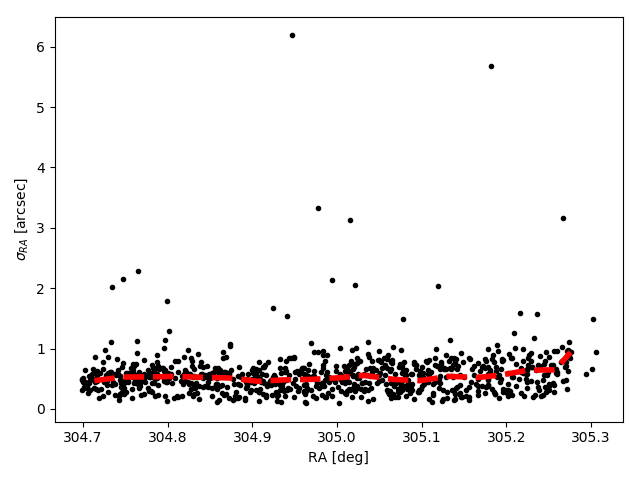
\includegraphics[width=0.475\linewidth]{./img/ra_delta_ra.png}
	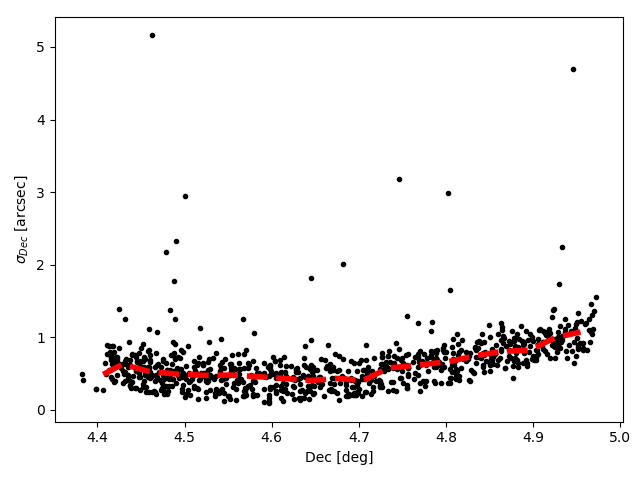
\includegraphics[width=0.475\linewidth]{./img/dec_delta_dec.png}
	\caption{Mean value of RA (left) and Dec (right) vs. the standard derivation with the median of the standard derivation (dashed red line)}
	\label{fig: realtive_coordinates}
\end{figure}
In Fig. \ref{fig: realtive_coordinates} the mean value of the coordinates vs the standard derivation is shown. The first noticeable feature is that the RA calibration looks better than the Dec calibration. Specially the median (red line) of the standard derivation is for RA calibration much more stable than for the Dec calibration. But in both cases only a small fraction of the sources ($\approx 1\%$) are above two pixel which means. Most of the sources have a standard derivation of around 0.5 arcsecs (or 0.25 pixel) which is OK.\\
The systematic effect in the Dec calibration is due to a large error in the second correction of the WCS. Currently it is not clear why this huge error happens because RA isn't effected by that.\\
\begin{figure}
	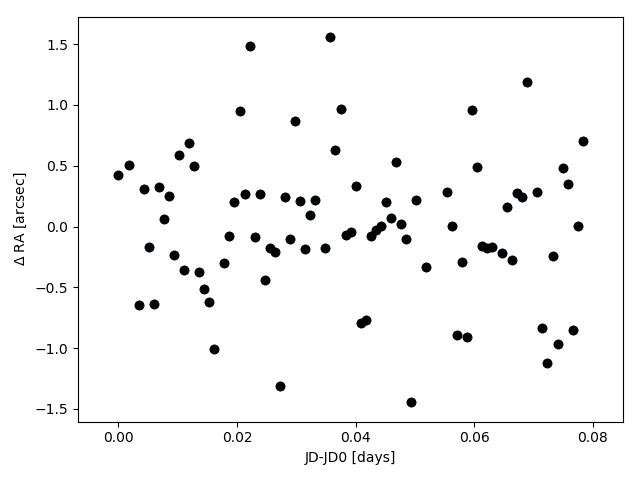
\includegraphics[width=0.475\linewidth]{./img/jd_delta_ra.png}
	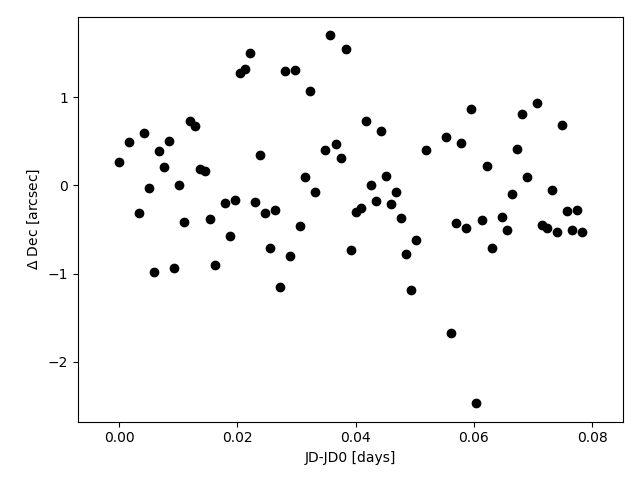
\includegraphics[width=0.475\linewidth]{./img/jd_delta_dec.png}
	\caption{Observation time vs. difference between RA and the mean RA (left) and between Dec and the mean Dec (right). $JD_0$ is the first JD of the observation run.}
	\label{fig: time_delta}
\end{figure}
Fig. \ref{fig: time_delta} shows the relative difference of RA and Dec of one source. As Fig. \ref{fig: realtive_coordinates} indicates most of the differences are below 1 arcsec. But we see also that there are outlayers with more than 1.5 arcsec difference to the mean value. That means that the calibration algorithm is not stable enough for some kind of images.

\begin{figure}
	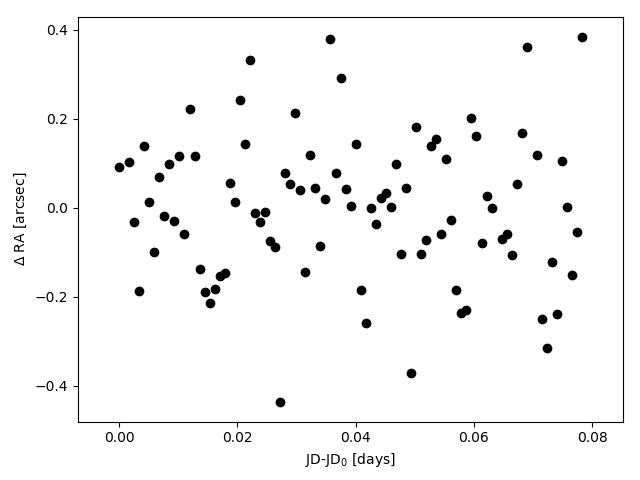
\includegraphics[width=0.475\linewidth]{./img/jd_delta_ra_all.png}
	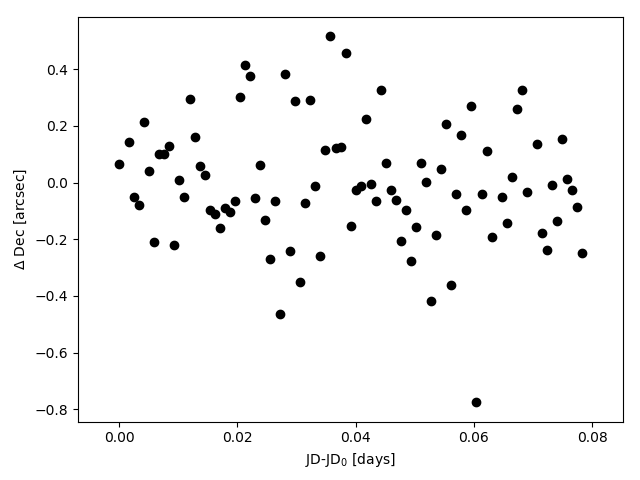
\includegraphics[width=0.475\linewidth]{./img/jd_delta_dec_all.png}
	\caption{Observation time vs. difference between RA and the mean RA (left) and between Dec and the mean Dec (right). Both are the mean values of all sources of one image}
	\label{fig: mean_coordiantes_diff}
\end{figure}
Also if we check the mean difference, we see in fig. \ref{fig: mean_coordiantes_diff} that most of the shifts are due to systematic shifts. This is easy to explain because a general shift correction of the WCS weren't done. Only one source was used to determine the center and if this source were for example a galaxy the position estimation could be unprecise. In one of the next updates a general shift correction will be included to correct this problem.